%%%%%%%%%%%%%%%%%%%%%%%%%%%%%%%%%%%%%%%%%%%%%%%%%%%%%%%%%%%%
%%  This Beamer template was created by Cameron Bracken.
%%  Anyone can freely use or modify it for any purpose
%%  without attribution.
%%
%%  Last Modified: January 9, 2009
%%

\documentclass[xcolor=x11names,compress]{beamer}

\usepackage{presitheme}
\author{Fabian Brix}
\date{July 30, 2013}

\begin{document}

\LLCornerWallPaper{0.2}{../resources/img/SignetUniBasel.pdf}

\begin{frame}
    \vspace*{\fill}
    \title[Bachelor Thesis]{Using Line Features for 3D Face Registration}
\subtitle{\scshape Bachelor Thesis Presentation}
    \author{Fabian Brix\\
        Department of Mathematics and Computer Science\\
        
\includegraphics[width=.4\textwidth]{../resources/img/LogoUniBasel.pdf}}
        \date{
            \today
        }
        \titlepage
    \vspace*{\fill}
    \end{frame}

%%%%%%%%%%%%%%%%%%%%%%%%%%%%%%%%%%%%%%%%%%%%%%%%%%%%%%
    \begin{frame}{Registration Overview}
        \begin{figure}
            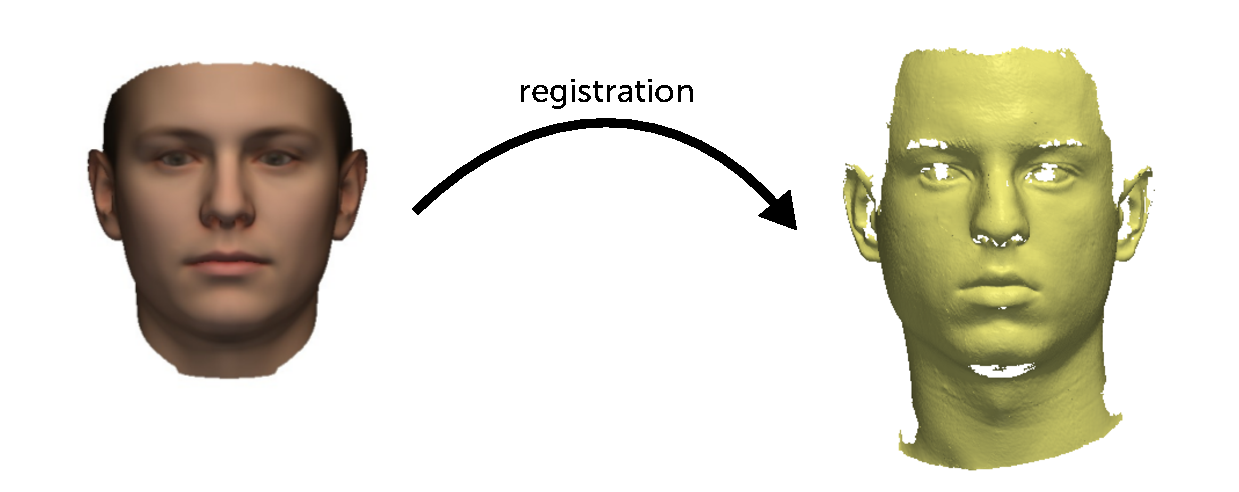
\includegraphics[width=\textwidth]{../resources/figures/intro1.pdf}
        \end{figure}
    \end{frame}

%%%%%%%%%%%%%%%%%%%%%%%%%%%%%%%%%%%%%%%%%%%%%%%%%%%%%%
    \begin{frame}{Registration Overview}
        \begin{figure}
            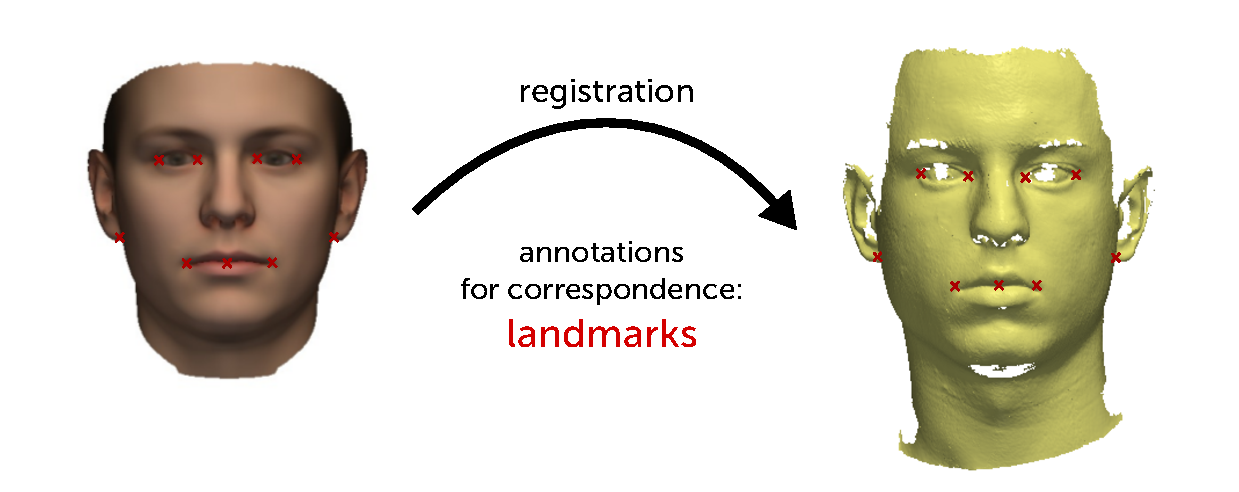
\includegraphics[width=\textwidth]{../resources/figures/intro2.pdf}
        \end{figure}
    \end{frame}

%%%%%%%%%%%%%%%%%%%%%%%%%%%%%%%%%%%%%%%%%%%%%%%%%%%%%%
    \begin{frame}{Registration Overview}
        \begin{figure}
            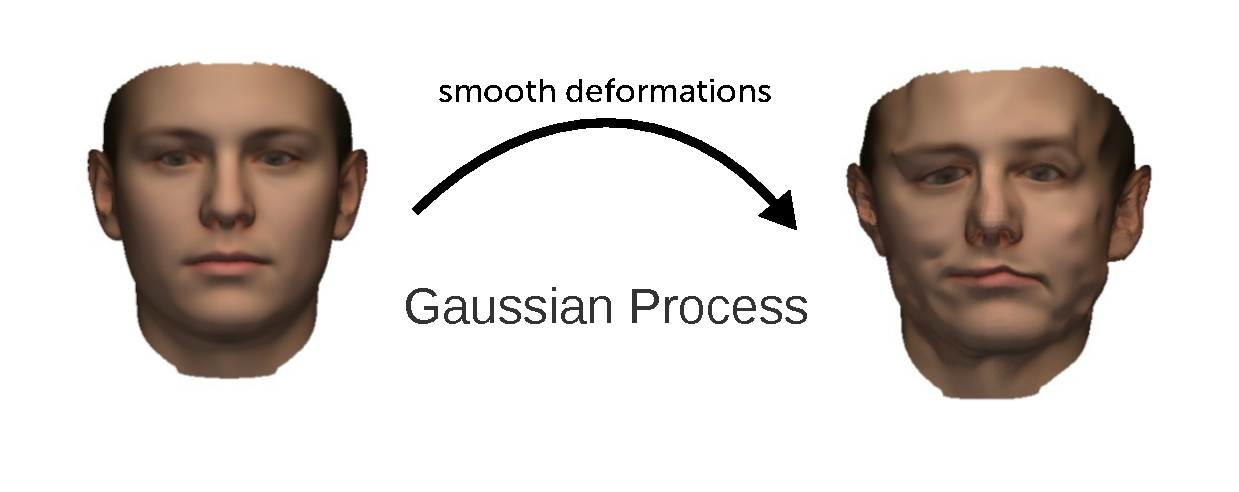
\includegraphics[width=\textwidth]{../resources/figures/intro3.pdf}
        \end{figure}
    \end{frame}

%%%%%%%%%%%%%%%%%%%%%%%%%%%%%%%%%%%%%%%%%%%%%%%%%%%%%%
    \begin{frame}{Registration Overview}
        \begin{figure}
            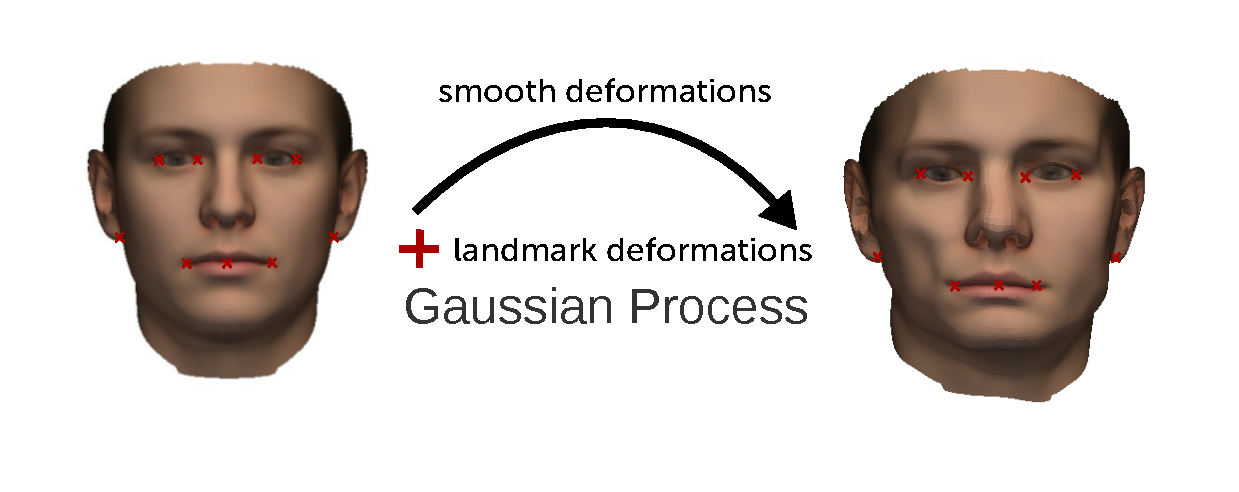
\includegraphics[width=\textwidth]{../resources/figures/intro4.pdf}
        \end{figure}
    \end{frame}


%%%%%%%%%%%%%%%%%%%%%%%%%%%%%%%%%%%%%%%%%%%%%%%%%%%%%%
    \begin{frame}{Registration Overview}
        \begin{figure}
            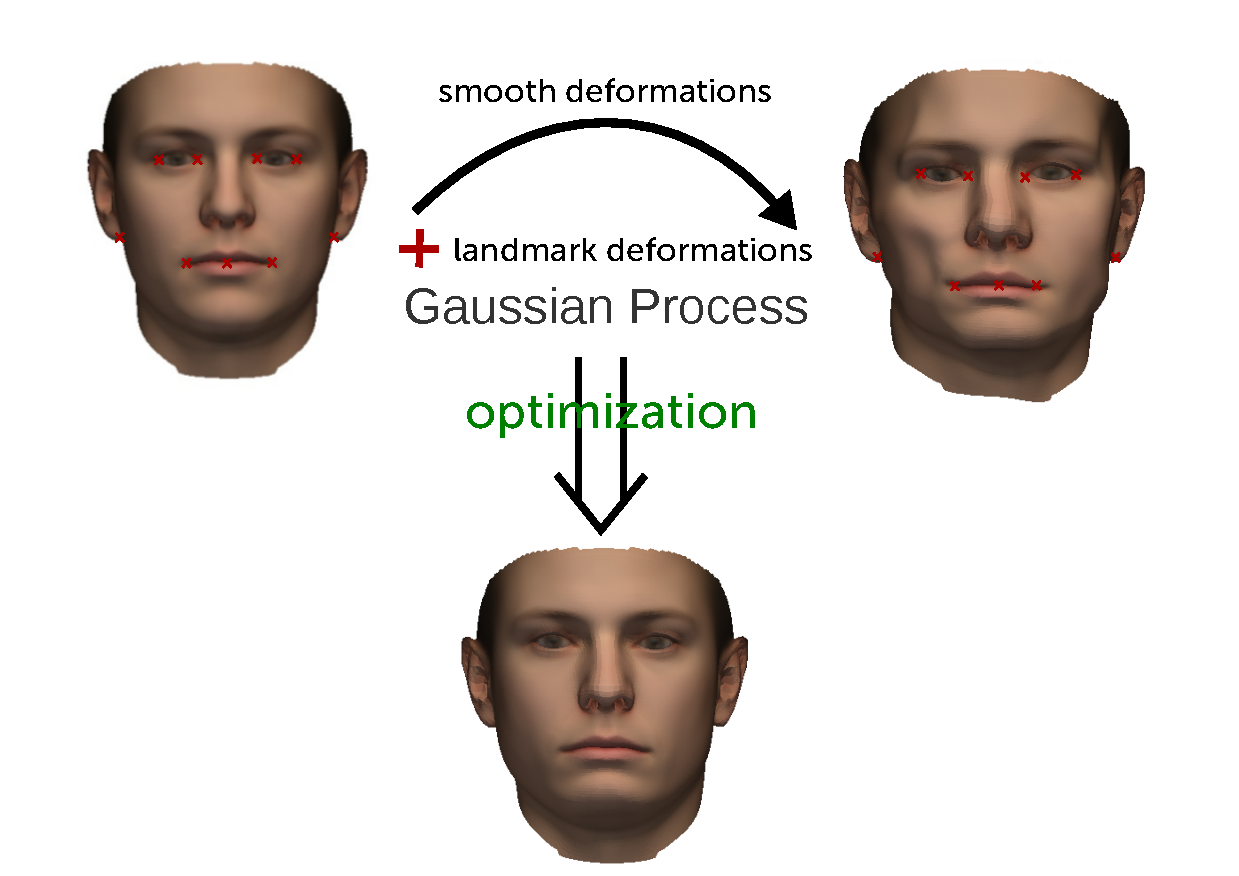
\includegraphics[width=\textwidth]{../resources/figures/intro5.pdf}
        \end{figure}
    \end{frame}

%%%%%%%%%%%%%%%%%%%%%%%%%%%%%%%%%%%%%%%%%%%%%%%%%%%%%%
    \begin{frame}{Registration Overview}
        \begin{figure}
            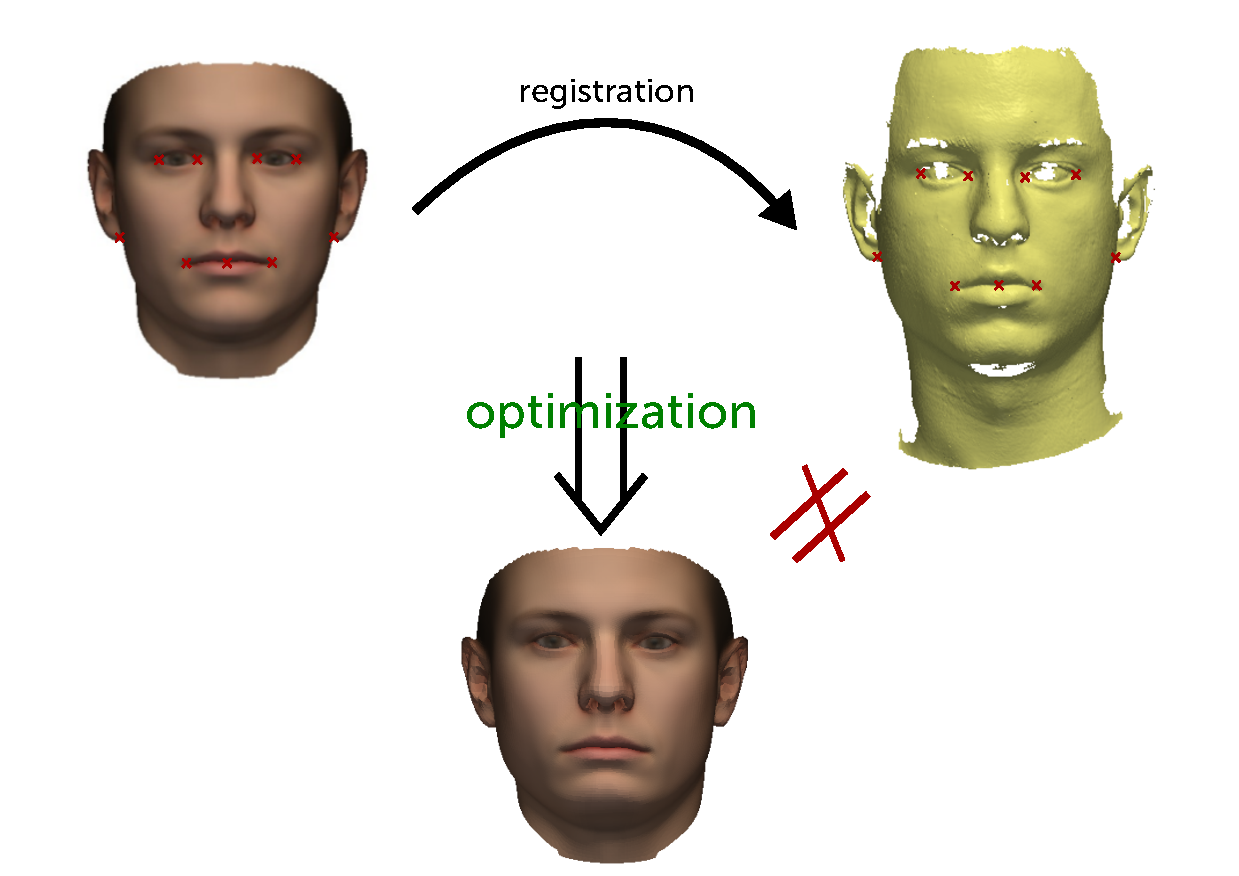
\includegraphics[width=\textwidth]{../resources/figures/intro6.pdf}
        \end{figure}
    \end{frame}

%%%%%%%%%%%%%%%%%%%%%%%%%%%%%%%%%%%%%%%%%%%%%%%%%%%%%%
    \begin{frame}{Registration Overview}
        \begin{figure}
            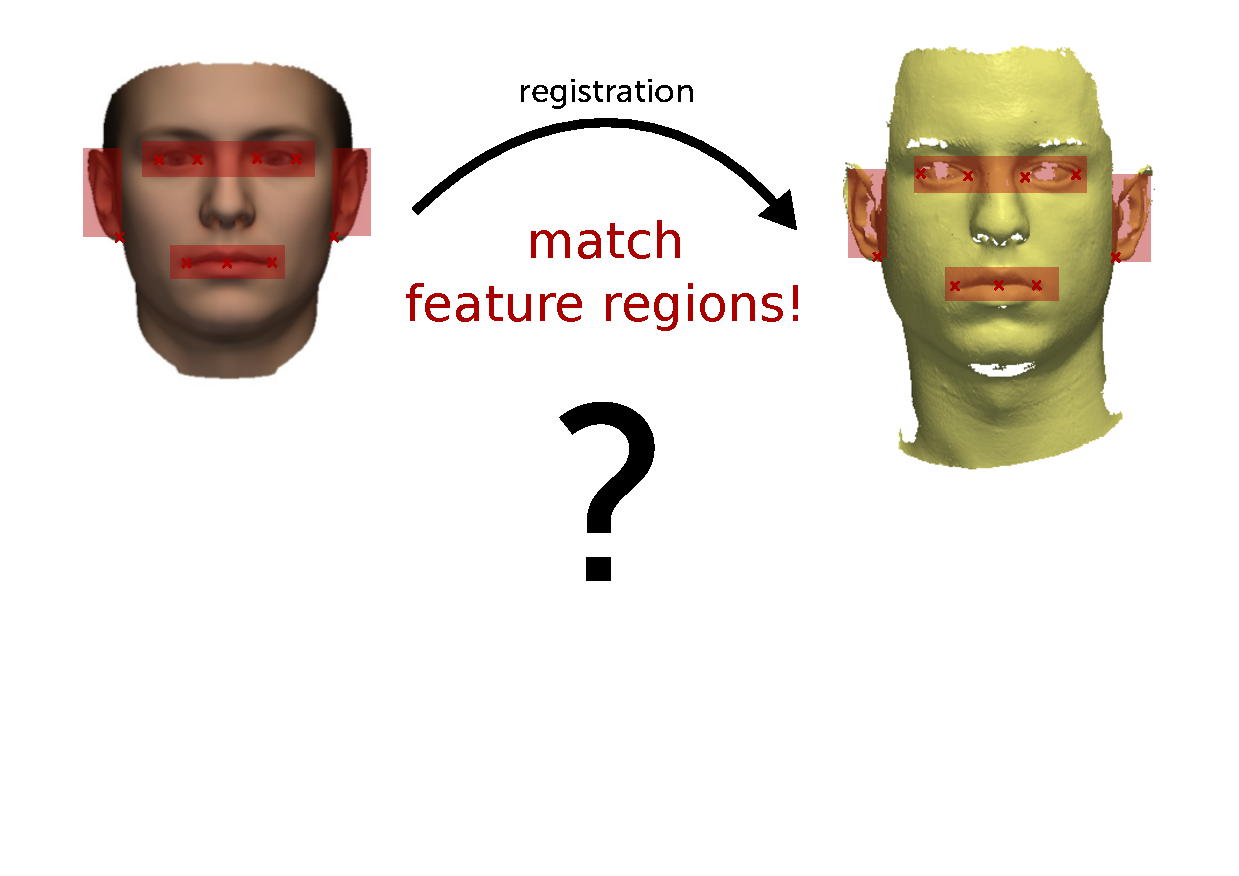
\includegraphics[width=\textwidth]{../resources/figures/intro7.pdf}
        \end{figure}
    \end{frame}

%%%%%%%%%%%%%%%%%%%%%%%%%%%%%%%%%%%%%%%%%%%%%%%%%%%%%%
    \begin{frame}{Outline}
        \tableofcontents
    \end{frame}

%%%%%%%%%%%%%%%%%%%%%%%%%%%%%%%%%%%%%%%%%%%%%%%%%%%%%%
%%%%%%%%%%%%%%%%%%%%%%%%%%%%%%%%%%%%%%%%%%%%%%%%%%%%%%
    \section{\scshape Data and Correspondence}
    \begin{frame}{Data and Correspondence}
        \begin{figure}
            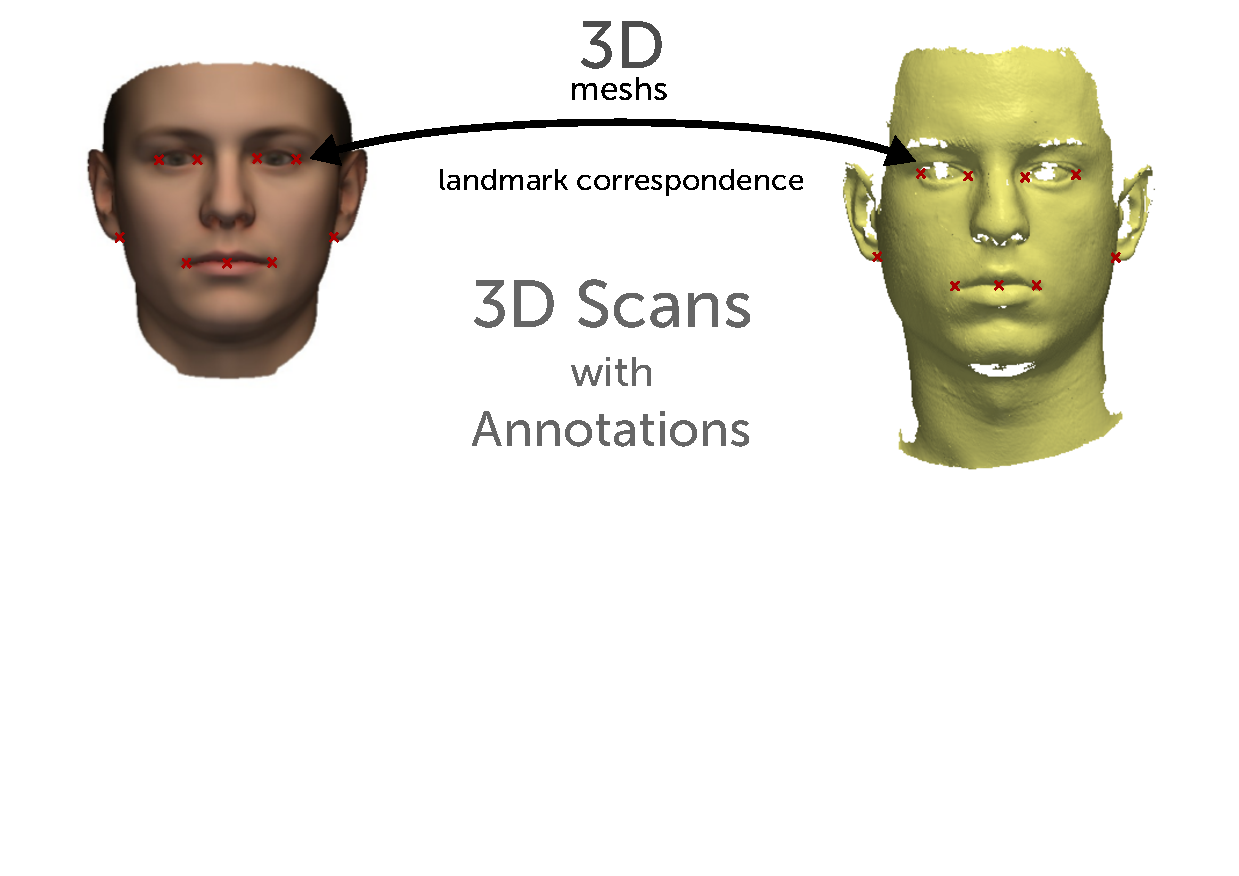
\includegraphics[width=.9\textwidth]{../resources/figures/givendata1.pdf}
        \end{figure}
    \end{frame}

%%%%%%%%%%%%%%%%%%%%%%%%%%%%%%%%%%%%%%%%%%%%%%%%%%%%%%
    \begin{frame}{Data and Correspondence}
        \begin{figure}
            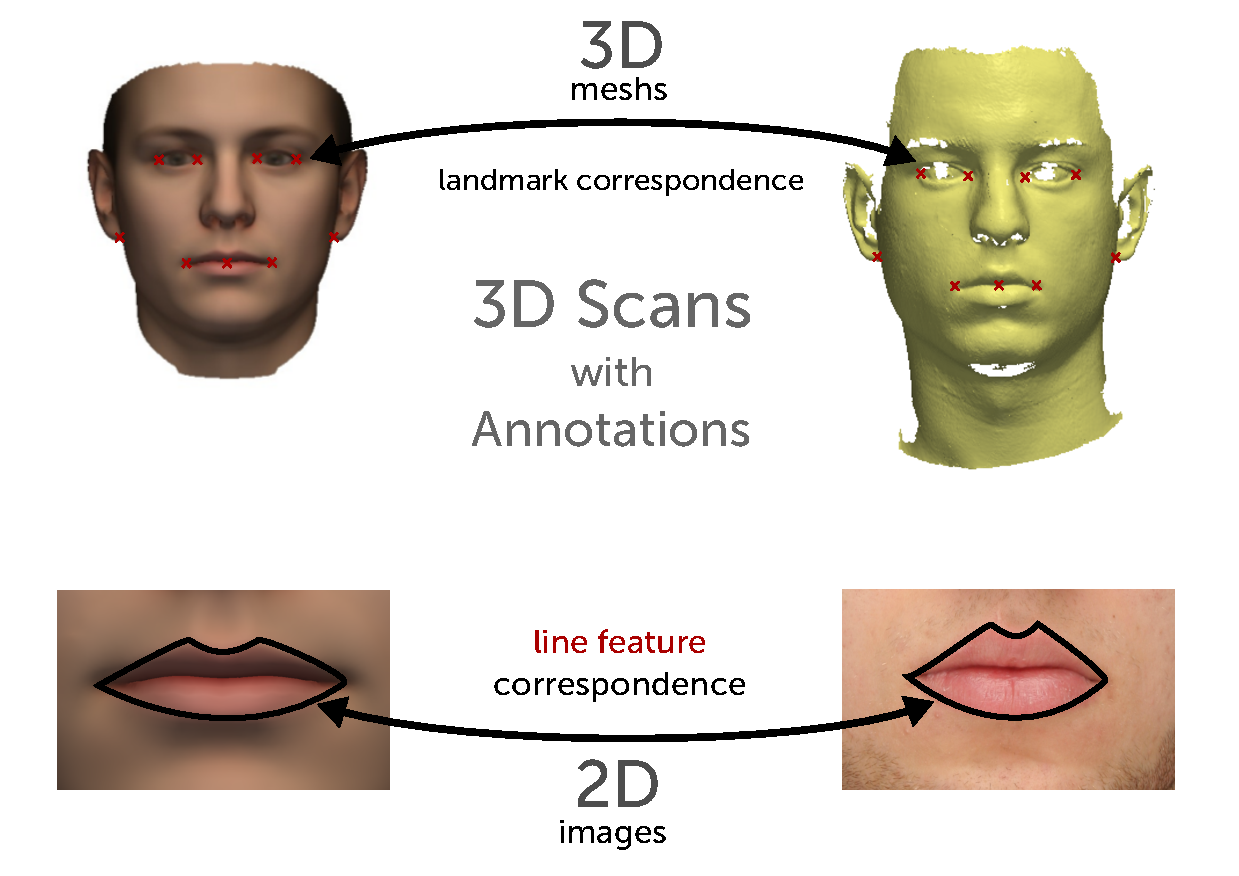
\includegraphics[width=.9\textwidth]{../resources/figures/givendata2.pdf}
        \end{figure}
    \end{frame}

%%%%%%%%%%%%%%%%%%%%%%%%%%%%%%%%%%%%%%%%%%%%%%%%%%%%%%
    \begin{frame}{Data and Correspondence}
        \begin{figure}
            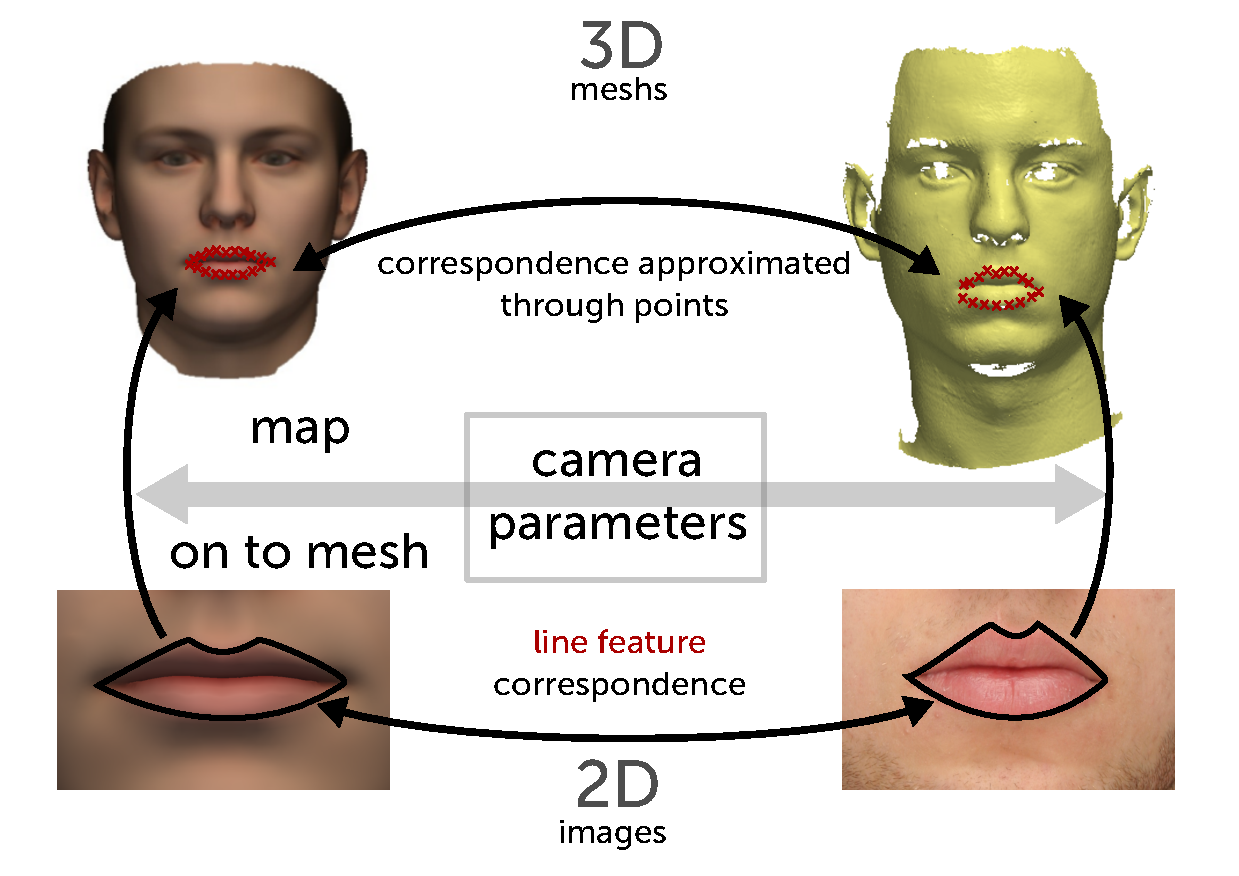
\includegraphics[width=.9\textwidth]{../resources/figures/givendata3.pdf}
        \end{figure}
    \end{frame}

%%%%%%%%%%%%%%%%%%%%%%%%%%%%%%%%%%%%%%%%%%%%%%%%%%%%%%
    \section{\scshape Using Line Features}
    \subsection{Sampling Line Features}
%%%%%%%%%%%%%%%%%%%%%%%%%%%%%%%%%%%%%%%%%%%%%%%%%%%%%%
    \begin{frame}{Mapping Line Features}
        Idea: Sample points from the line features and use them as additional landmarks
        \begin{figure}
            \centering
            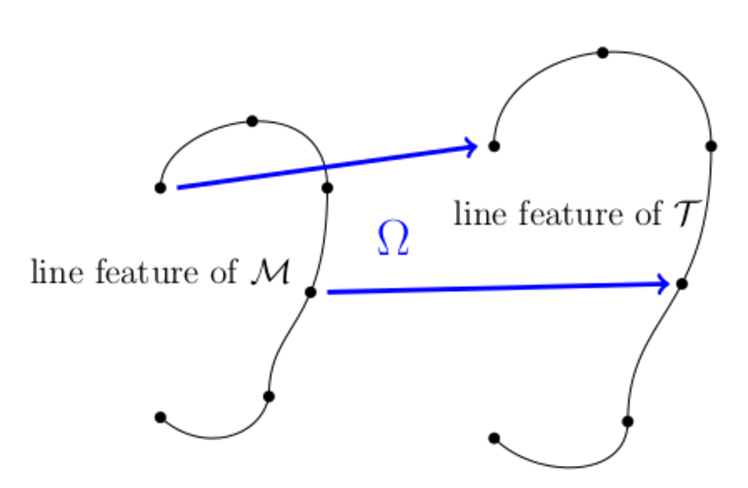
\includegraphics[width=.5\textwidth]{../resources/img/linefeaturemapping.pdf}
        \end{figure}
        What about correspondence?
    \end{frame}

%%%%%%%%%%%%%%%%%%%%%%%%%%%%%%%%%%%%%%%%%%%%%%%%%%%%%%
    \begin{frame}{Equidistant Sampling}
        Approximate correspondance by sampling line features in equidistant intervals
        \begin{figure}
            \centering
            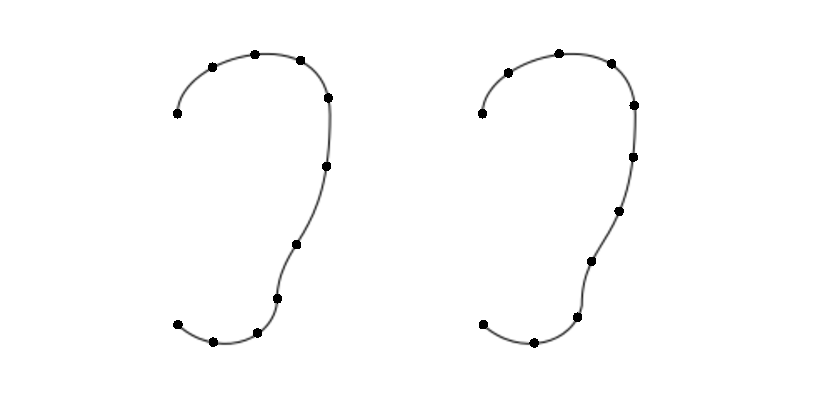
\includegraphics[width=.7\textwidth]{../resources/figures/ears_diffparam.pdf}
        \end{figure}
    \end{frame}

%%%%%%%%%%%%%%%%%%%%%%%%%%%%%%%%%%%%%%%%%%%%%%%%%%%%%%
    \begin{frame}{B\'{e}zier curves}
        Problem: Line features consist of B\'{e}zier curve segments\\
        underlying parameter t is not linear

        Approximate arc-length of curve through euclidean distance of sampled points
        \begin{figure}
            \centering
            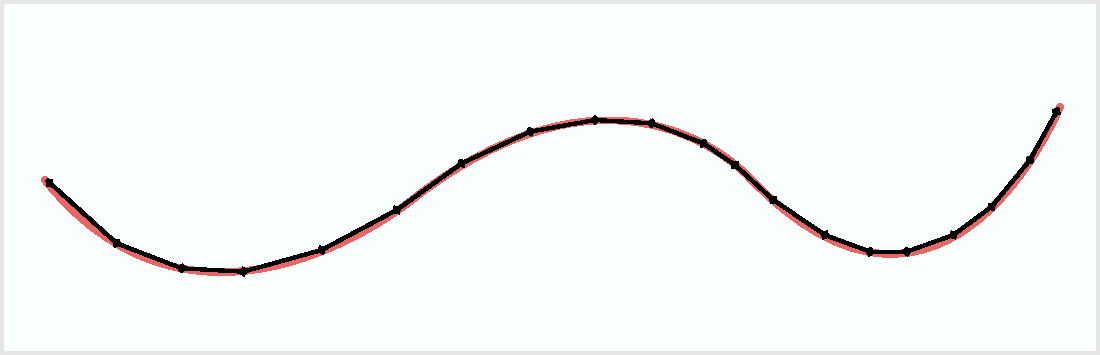
\includegraphics[width=.7\textwidth]{../resources/figures/distance_computation.pdf}
        \end{figure}
        $\rightarrow$ map point coordinates to approximated fractional length of curve
    \end{frame}

%%%%%%%%%%%%%%%%%%%%%%%%%%%%%%%%%%%%%%%%%%%%%%%%%%%%%%
    \subsection{Projection: 2D to 3D}
    \begin{frame}{Pipeline: Projection}
        \begin{figure}   
            \centering
            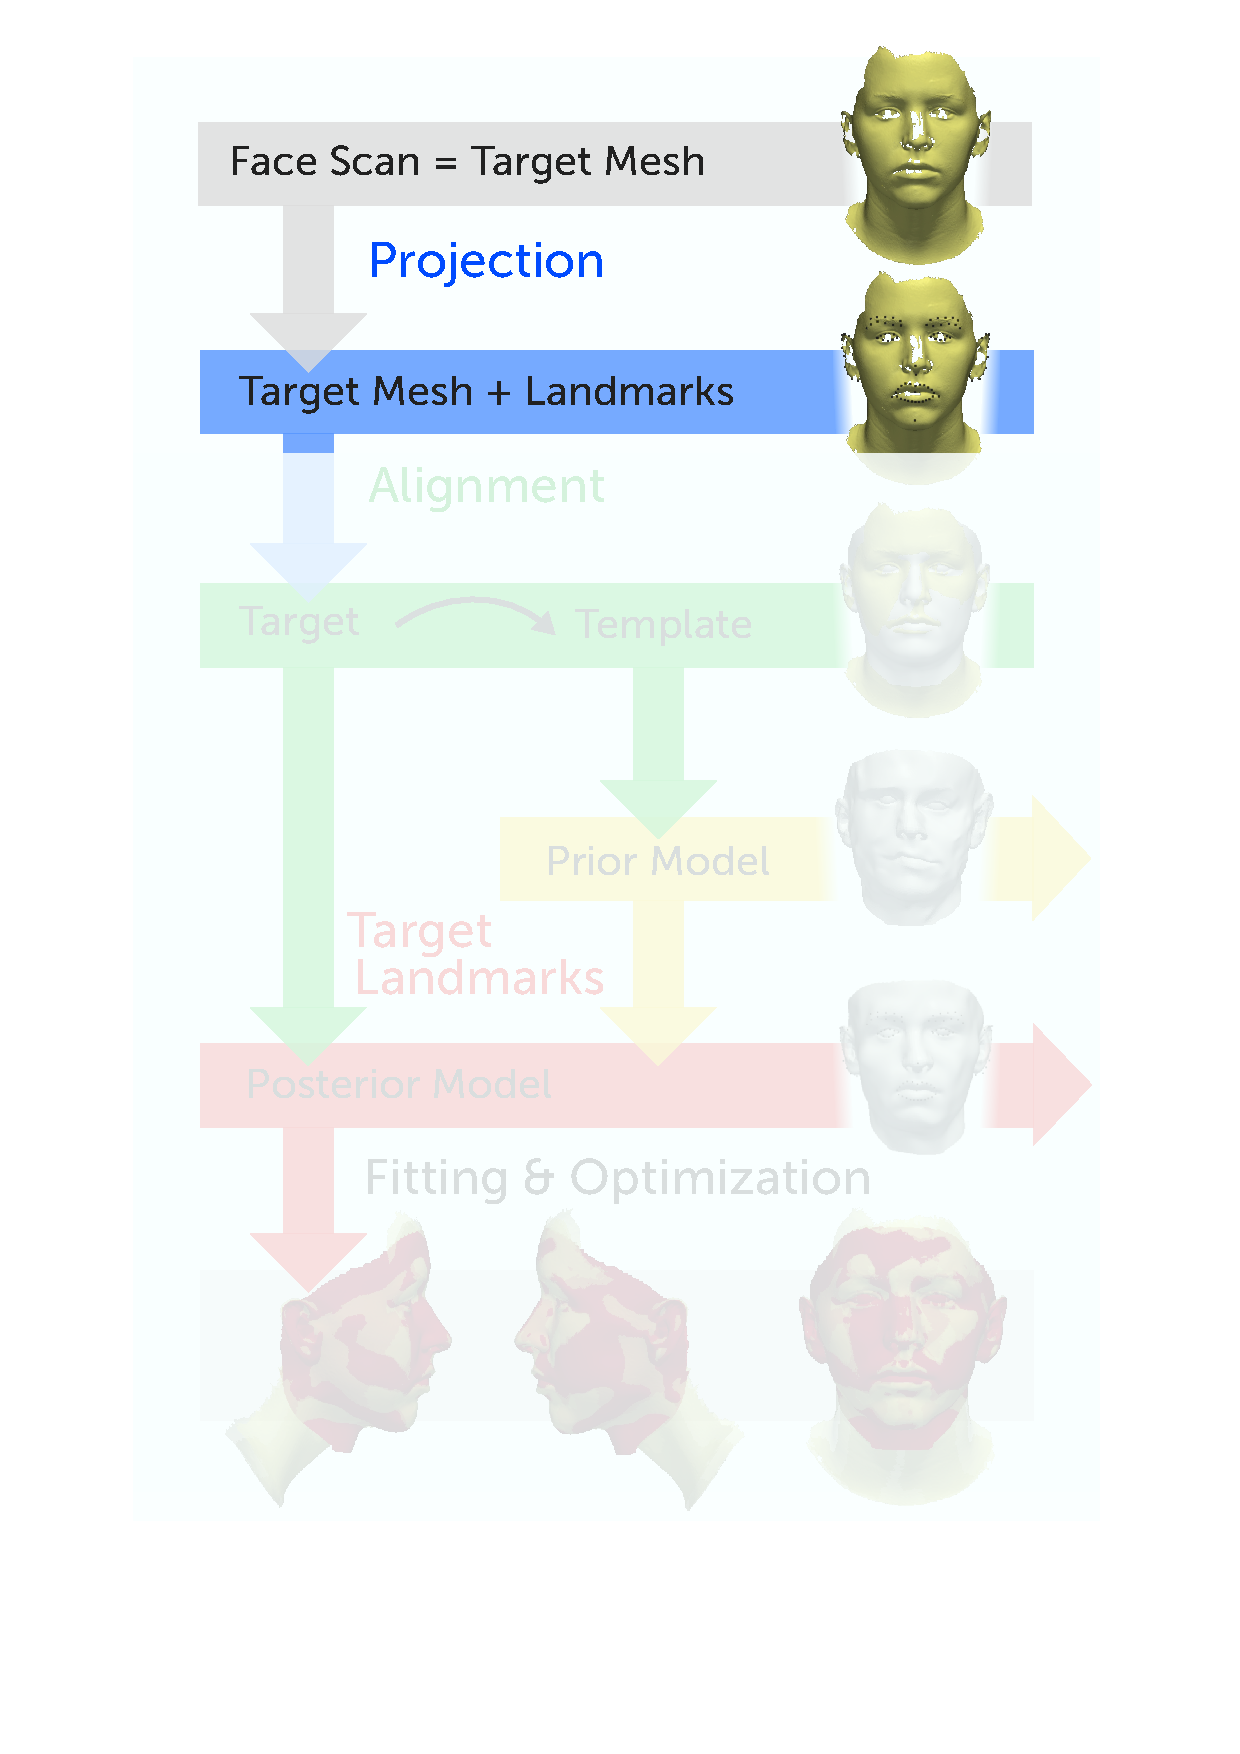
\includegraphics[width=.6\textwidth]{../resources/figures/pipeline_projection.pdf}
        \end{figure}
    \end{frame}

    \begin{frame}{Projection: 2D to 3D}
        \begin{figure}
            \centering
            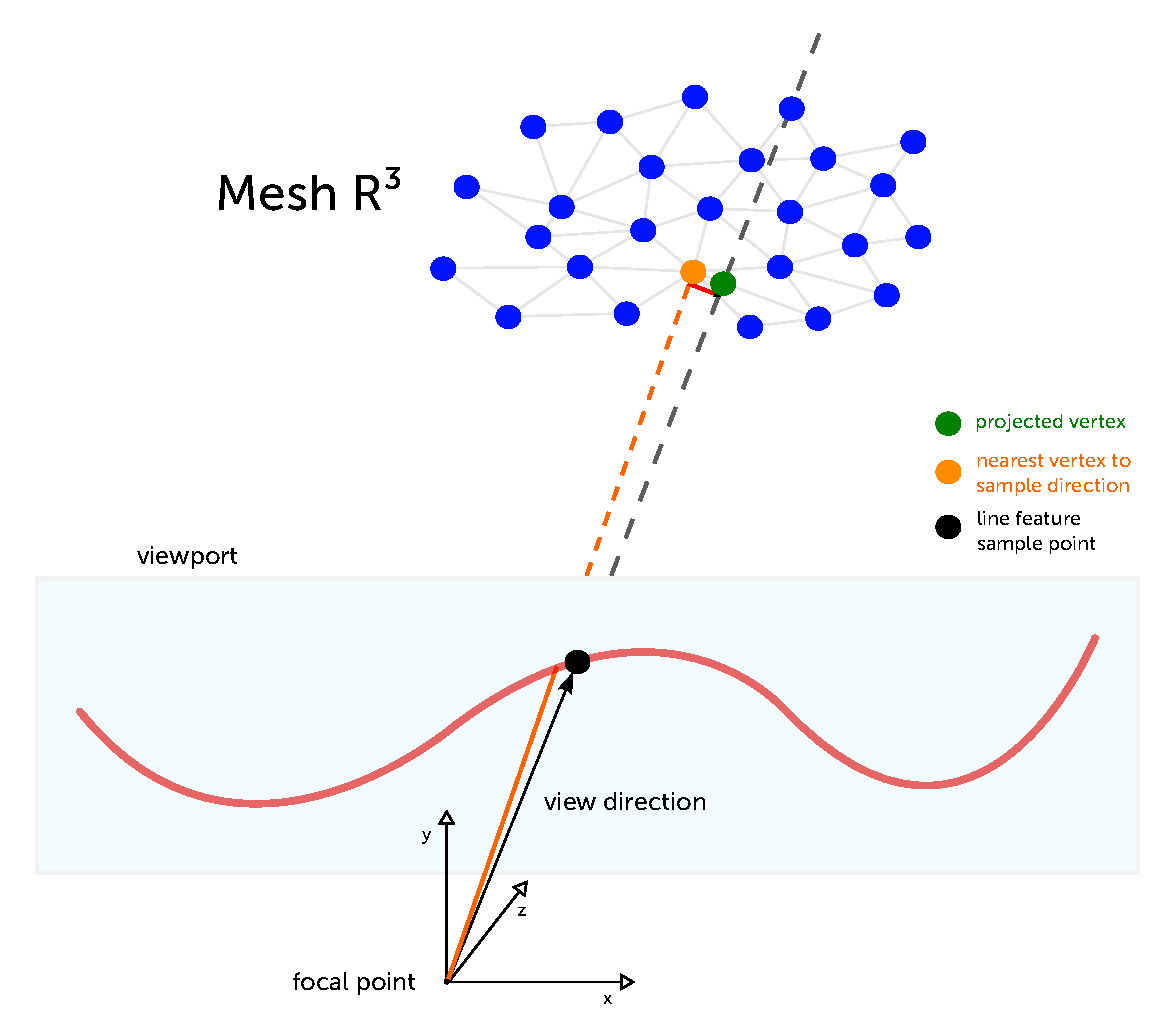
\includegraphics[width=.8\textwidth]{../resources/figures/projection.pdf}
        \end{figure}
    \end{frame}

    \begin{frame}{Projection: holes}
        \begin{figure}
            \centering
            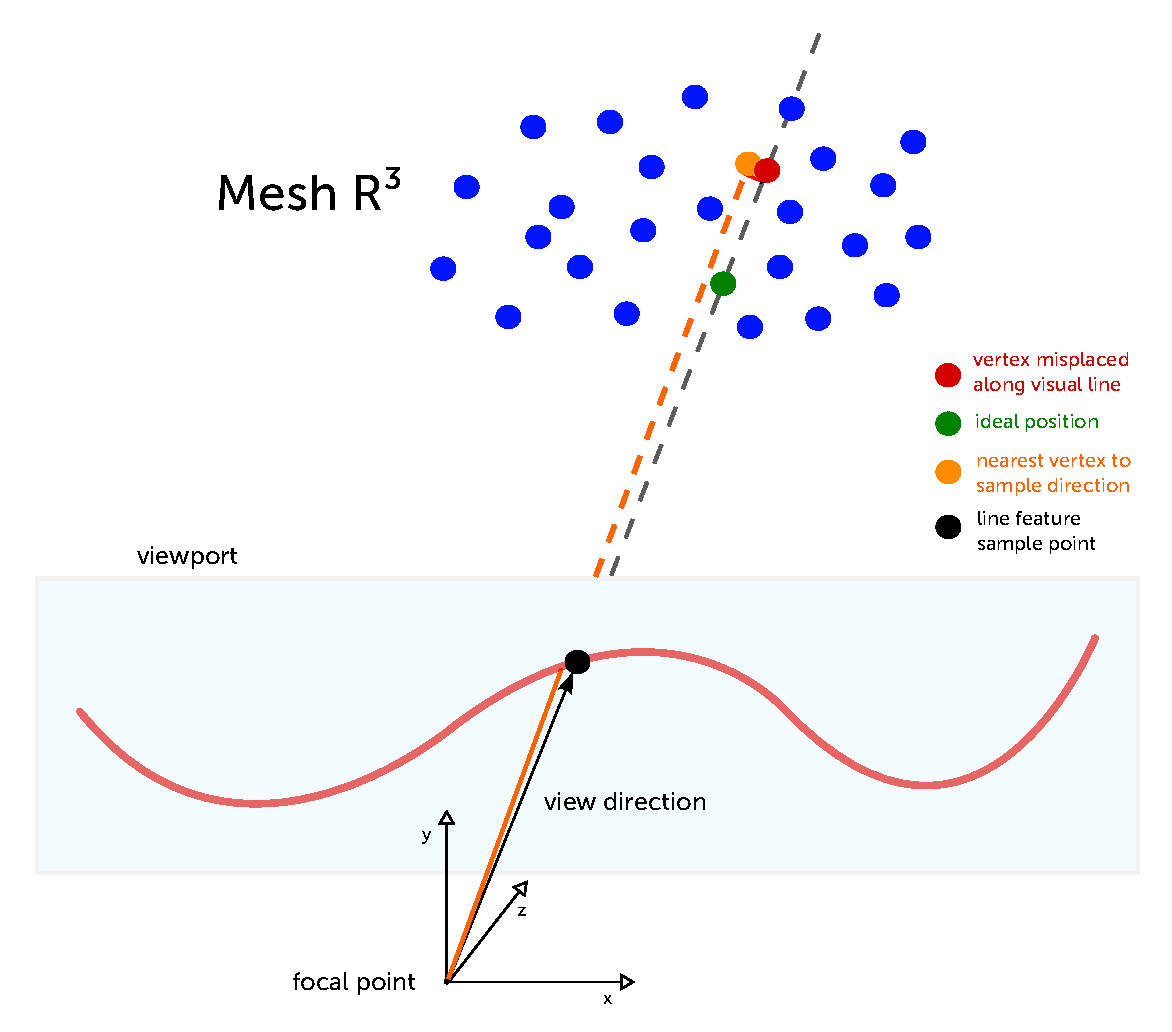
\includegraphics[width=.8\textwidth]{../resources/figures/projection_holes.pdf}
        \end{figure}
    \end{frame}


    \subsection{Results of 3D representation}
    \begin{frame}{Results of 3D representation}
        show images of projected line features
    \end{frame}

    \begin{frame}{Template/Target Alignment}
        \begin{figure}   
            \centering
            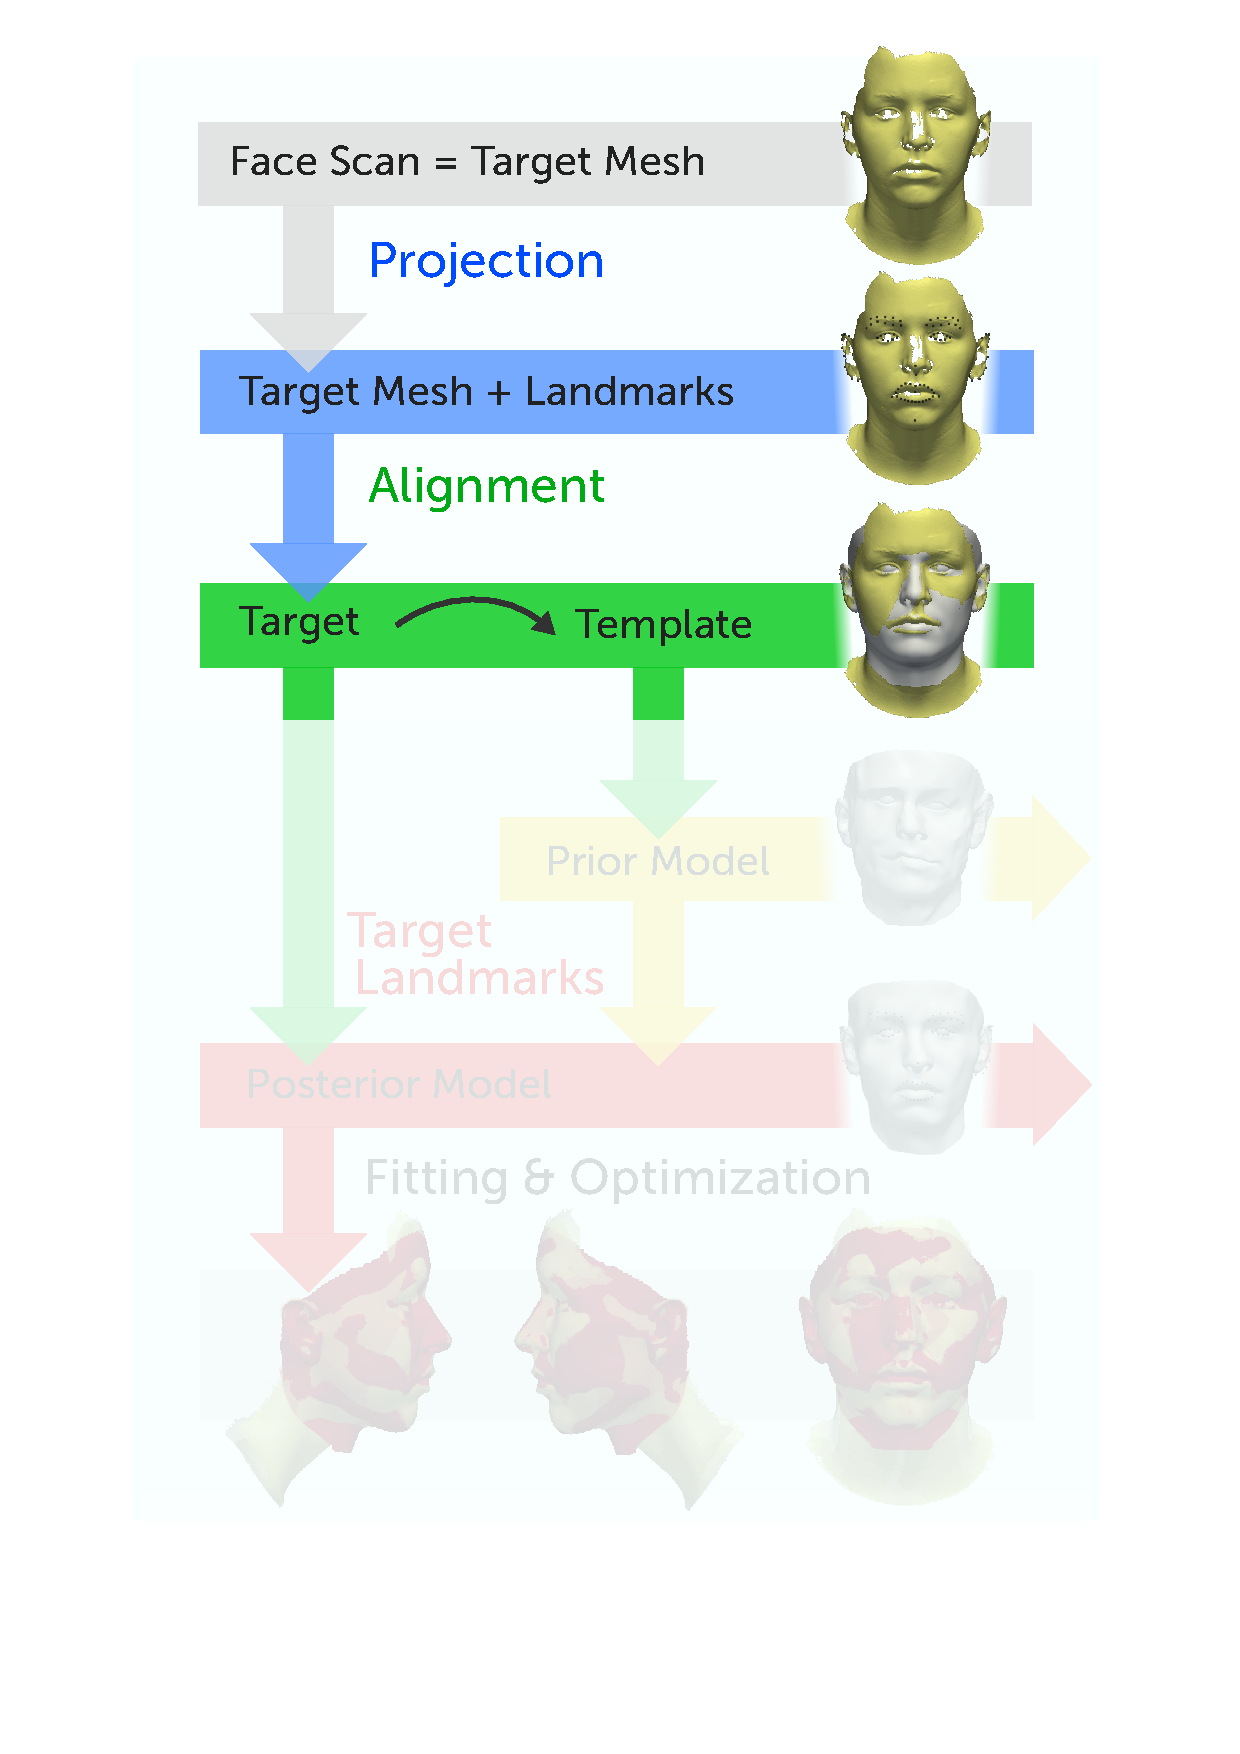
\includegraphics[width=.6\textwidth]{../resources/figures/pipeline_alignment.pdf}
        \end{figure}
    \end{frame}

%%%%%%%%%%%%%%%%%%%%%%%%%%%%%%%%%%%%%%%%%%%%%%%%%%%%%%
%%%%%%%%%%%%%%%%%%%%%%%%%%%%%%%%%%%%%%%%%%%%%%%%%%%%%%
    \section{\scshape Gaussian Process Regression}
    \subsection{Gaussian Process}
    \begin{frame}{Gaussian Process}
        a stochastic process where a finite set of random variables has a normal distribution
        defined by mean and covariance function

        \begin{align*}
            GP \sim (\mu, \Sigma)
        \end{align*}
    \end{frame}

%%%%%%%%%%%%%%%%%%%%%%%%%%%%%%%%%%%%%%%%%%%%%%%%%%%%%%
    \subsection{GP Prior}
    \begin{frame}{GP Prior}
        view Gaussian Process as a distribution over functions,\\
        each random variable represents possible function values at specified input points
        $\mu : \mathbb{R} \rightarrow 0$ to simplify computations

        \begin{figure}
            \centering
            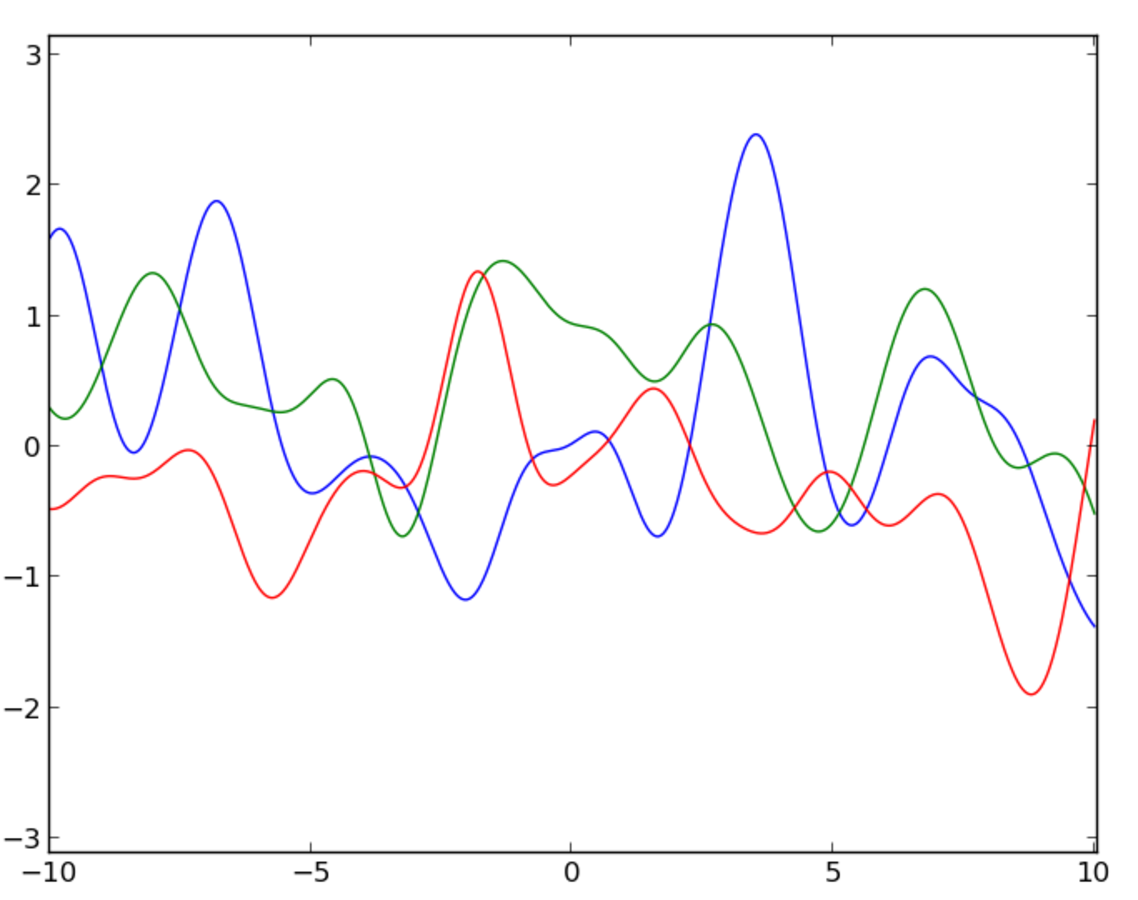
\includegraphics[width=.6\textwidth]{../resources/figures/gp_prior.pdf}
            \caption{normal distribution over 1000 input points}
        \end{figure}

    \end{frame}

%%%%%%%%%%%%%%%%%%%%%%%%%%%%%%%%%%%%%%%%%%%%%%%%%%%%%%
    \subsection{GP Posterior}
    \begin{frame}{GP Posterior}
        infer a set of possible functions by conditioning the distribution on the outputs $y_{i}$ of a training set
        \begin{equation*}
            S = \{(x_{1}, y_{1}), \cdots, (x_{n},y_{n})\}
        \end{equation*}
        add noise $y = f(x) + \varepsilon$?
    \end{frame}

\begin{frame}{Joint Distribution}
\begin{equation*}
\begin{bmatrix}\textbf{f}\\\textbf{f}_{*}\end{bmatrix}
\sim \mathcal{N}\left(\textbf{0},
\begin{bmatrix}
    \Sigma(X) & \Sigma(X,X_{*})\\
    \Sigma(X_{*},X) & \Sigma(X_{*})\\
\end{bmatrix}
\right)
\end{equation*}
\end{frame}

\begin{frame}{Posterior Distribution}
\begin{align*}
 & p(\textbf{f}_{*}\vert\textbf{f} =\textbf{y})
 & \mu = 
 & K = 
\end{align*}

\begin{figure}
\centering
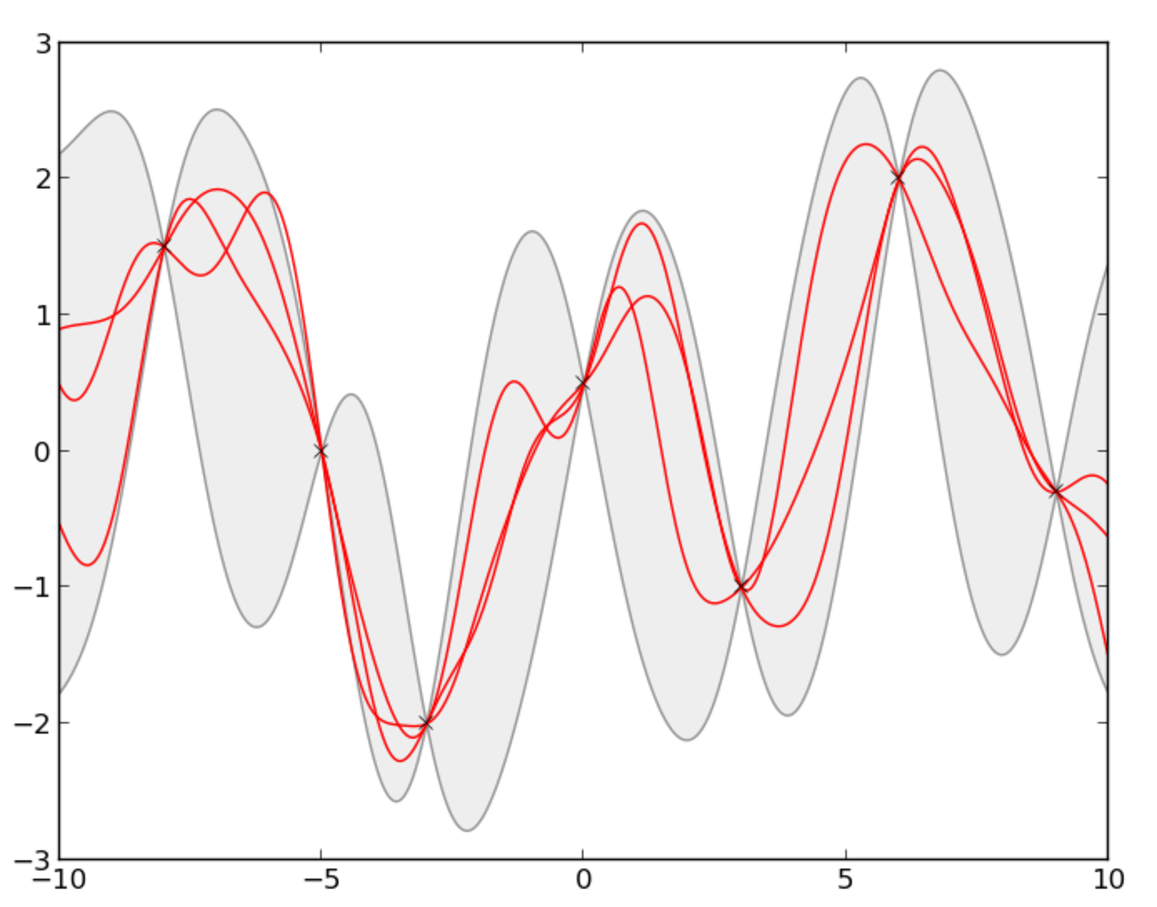
\includegraphics[width=.6\textwidth]{../resources/figures/gp_posterior.pdf}
\caption{posterior distribution fixed at 7 input points}
\end{figure}
\end{frame}

%%%%%%%%%%%%%%%%%%%%%%%%%%%%%%%%%%%%%%%%%%%%%%%%%%%%%%
%%%%%%%%%%%%%%%%%%%%%%%%%%%%%%%%%%%%%%%%%%%%%%%%%%%%%%
\subsection{Application to 3D Face Registration}
\begin{frame}{GPR in 3D Face Registration}
definition of Vector-valued GP
\begin{align*}
& \mu: \mathbb{R}^3 \rightarrow \mathbb{R}^3\\
& k: \mathbb{R}^3 \rightarrow \mathbb{R}^3 \times \mathbb{R}^3
\end{align*}
\end{frame}

\begin{frame}{Pipeline: Deformation Prior}
\begin{figure}   
\centering
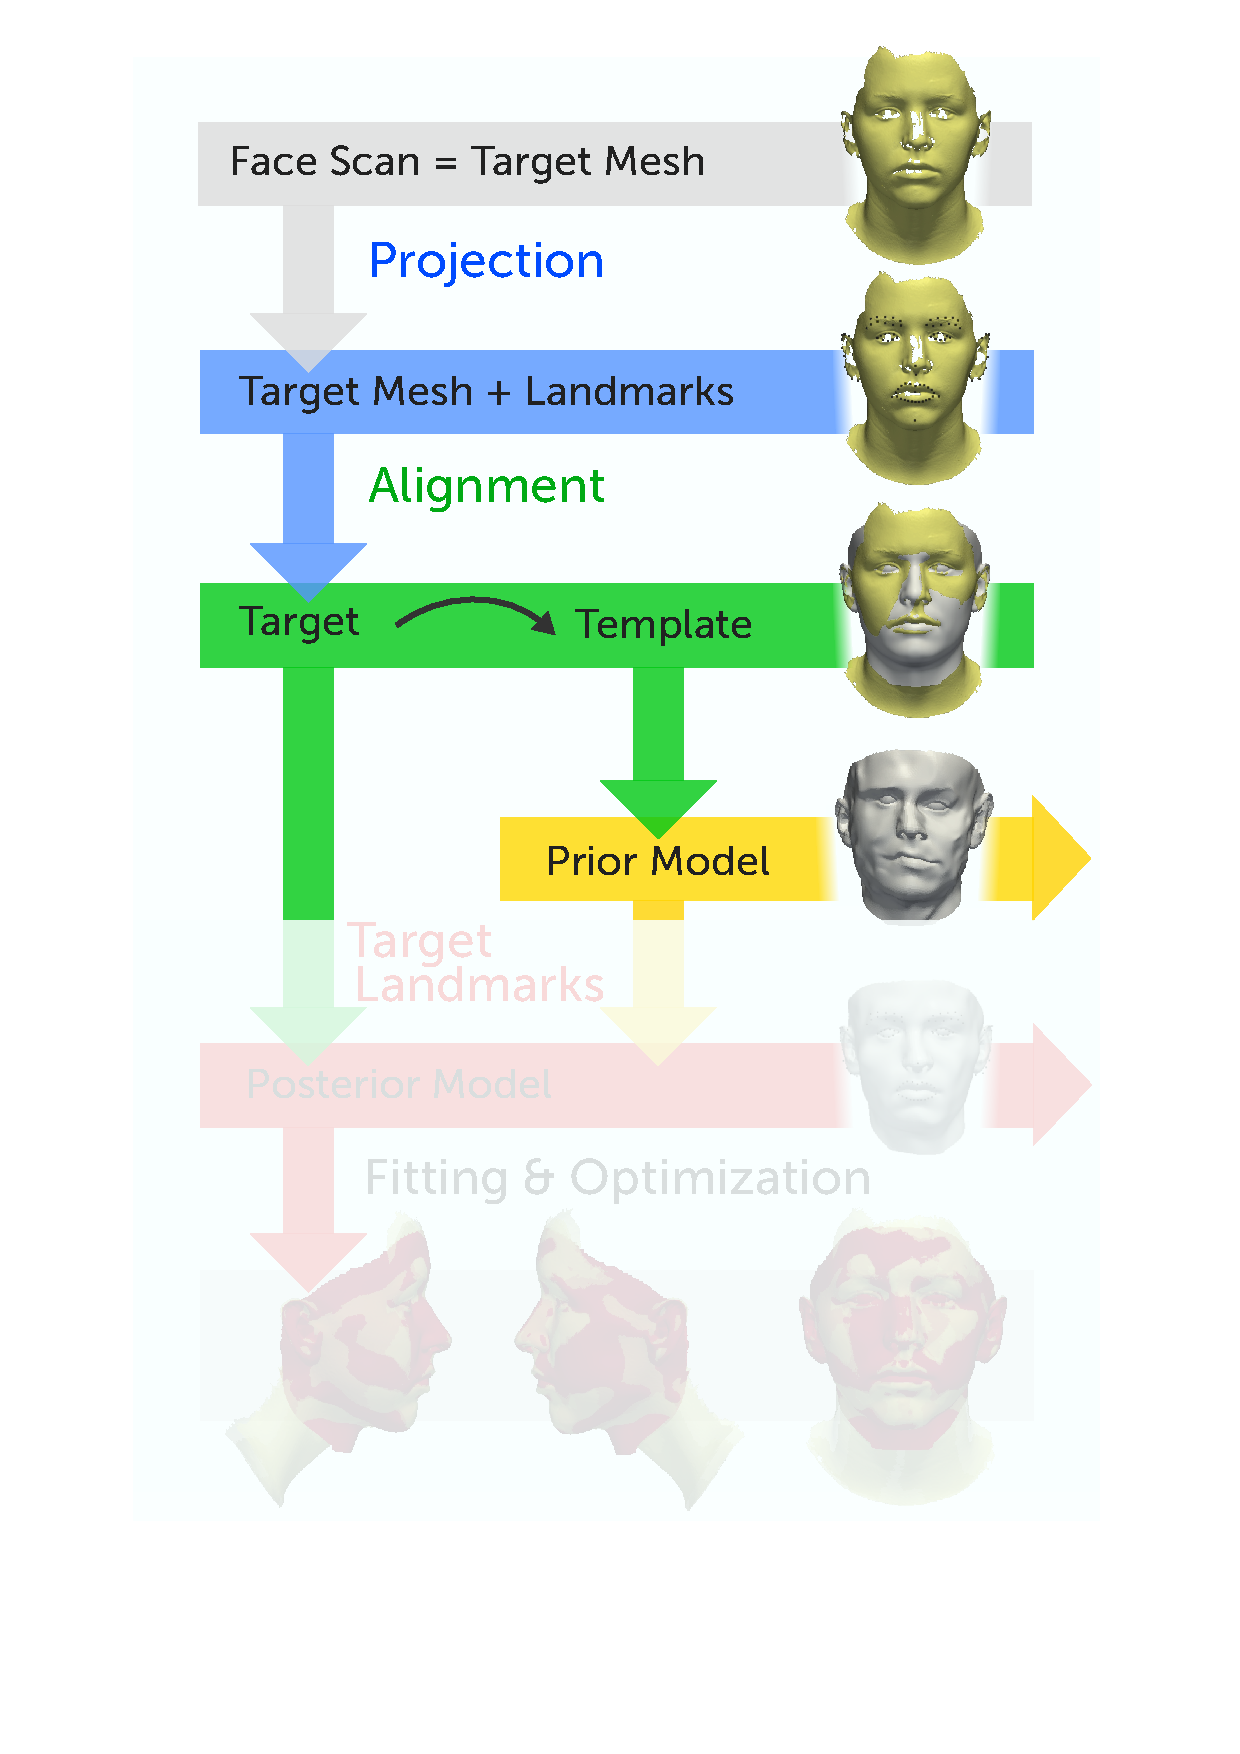
\includegraphics[width=.6\textwidth]{../resources/figures/pipeline_prior.pdf}
\end{figure}
%\begin{comment}
%projected line features on to face scans and template/mean mesh, now we want to define a prior distribution on the template mesh
%\end{comment}
\end{frame}

%%%%%%%%%%%%%%%%%%%%%%%%%%%%%%%%%%%%%%%%%%%%%%%%%%%%%%
\begin{frame}{Deformation Prior}
build GP Prior from template mesh vertices\\
$\rightarrow$ GP defines deformation on every vertex of the template
\begin{figure}
    \centering
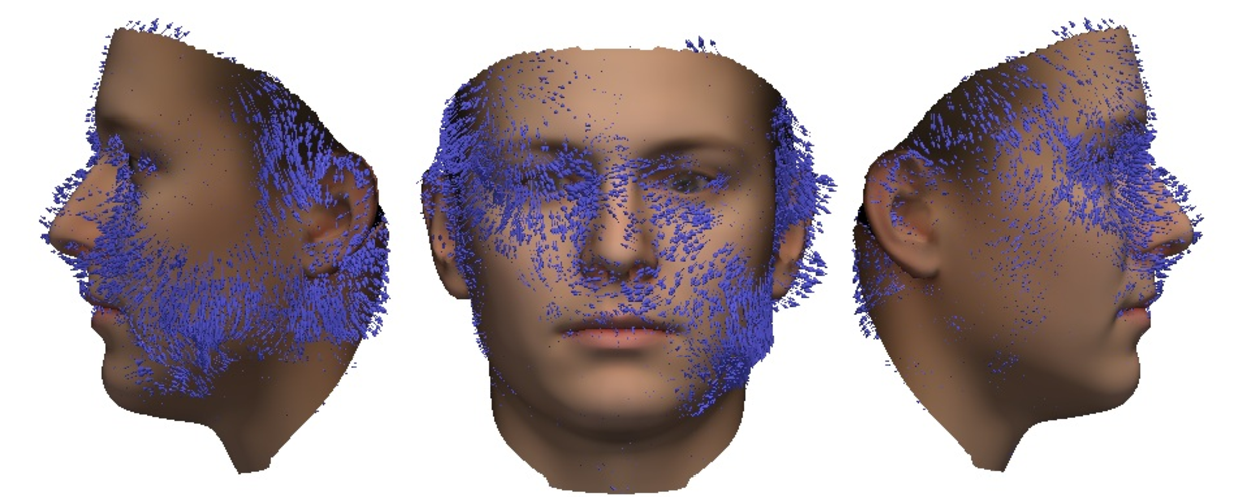
\includegraphics[width=.6\textwidth]{../resources/img/prior_deformations.pdf}
\end{figure}
\end{frame}

%%%%%%%%%%%%%%%%%%%%%%%%%%%%%%%%%%%%%%%%%%%%%%%%%%%%%%
\begin{frame}{Pipeline: Deformation Posterior}
\begin{figure}   
\centering
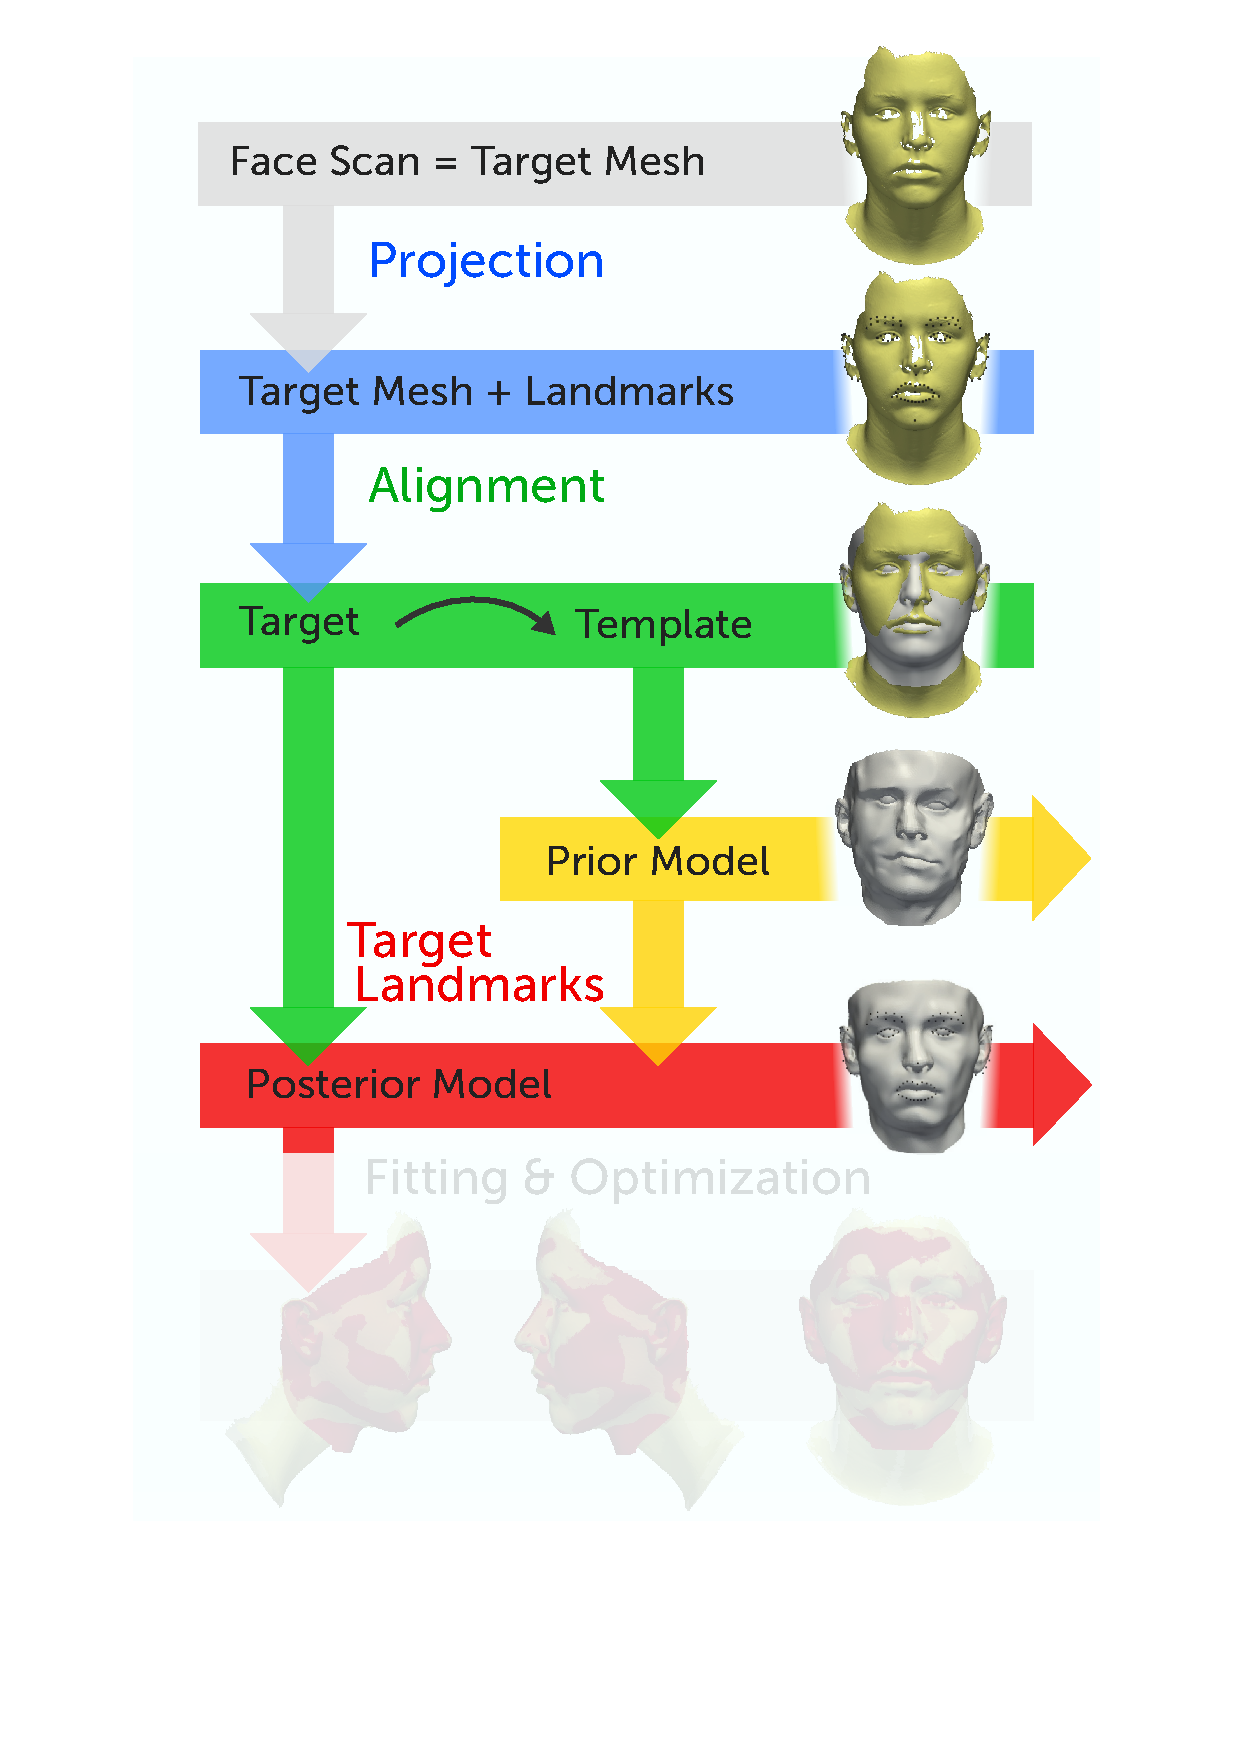
\includegraphics[width=.6\textwidth]{../resources/figures/pipeline_posterior.pdf}
\end{figure}
%\begin{comment}
%defined prior deformations on the template!
%now incorporate line features as additional landmarks.
%\end{comment}
\end{frame}

%%%%%%%%%%%%%%%%%%%%%%%%%%%%%%%%%%%%%%%%%%%%%%%%%%%%%%
\begin{frame}{3D GP Posterior}
Training data for inference in the space of possible template surface deformations:\\
comprised of the residuals of the line feature sample coordinates        
\begin{equation*}
R = \{t - m \vert t \in L_{T}, l \in L_{M}\} 
\end{equation*}
\begin{figure}   
\centering
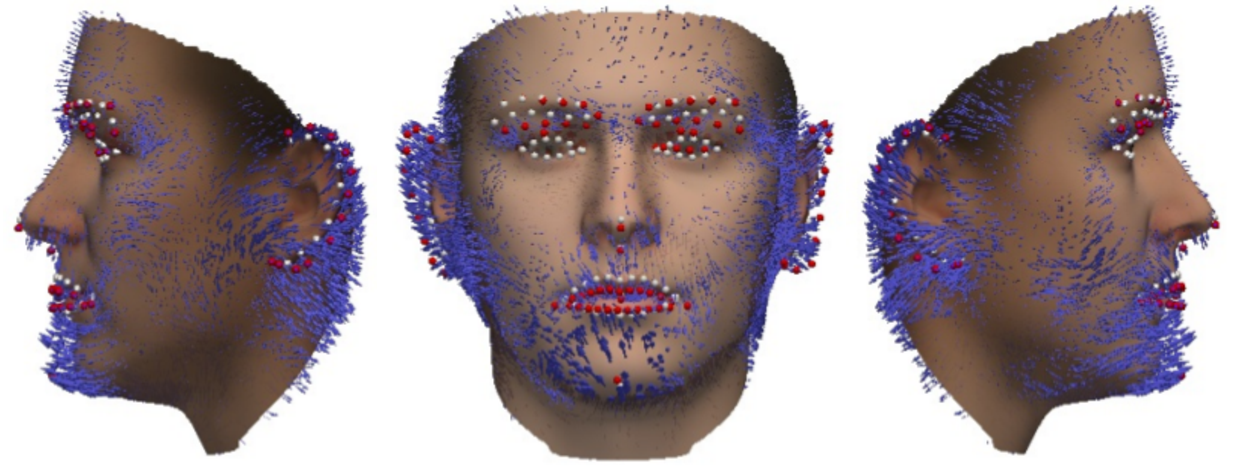
\includegraphics[width=.6\textwidth]{../resources/img/posterior_deformations.pdf}
\end{figure}

\end{frame}

\begin{frame}{Posterior Meshs}
    \begin{figure}
        \centering
        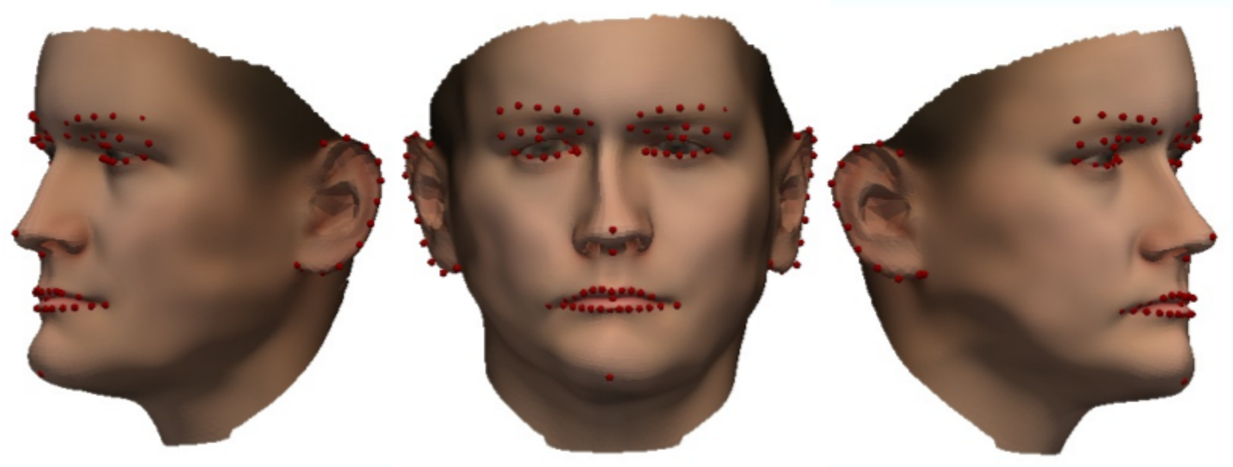
\includegraphics[width=.6\textwidth]{../resources/img/posterior_sample_17.pdf}
    \end{figure}
\end{frame}

\subsection{Optimization}
\begin{frame}{Parametric Model}
    GP Posterior distribution of admissible deformations\\
    How to optimize deformation samples?\\
    Mercer's theorem: distribution $\rightarrow$ parametric model\\
    $\rightarrow$ optimize model parameters
\end{frame}

\begin{frame}{Loss function}

\end{frame}

\begin{frame}{Robust Estimators}
\end{frame}

\section{Results}
\begin{frame}{Results}

\end{frame}
\end{document}
